\section{Let Míčku}
\label{ssec:let-micku}
Let míčku se často zjednodušuje a zanedbávají se některé síly, které na letící
míček působí. Když uvážíme jen gravitaci zjistíme, že by míček za letu měl
dráhou opsat parabolu. Pro kratší dobu letu a velkou rychlost tento předpoklad
není nikterak škodlivý.\footnote{Jako tomu bývá často právě ve stolním tenisu}.
Tyto síly můžeme vidět na rovnici \myref{rovnici}{eq:Newton} a na
\myref{obrázku}{fig:let-micku}.

\myref{Rovnice}{eq:Newton} získáme, když si rozepíšeme 2. Newtonův kinematický
zákon. 
\begin{equation}
 \label{eq:Newton}
  \vec{F_g} + \vec{v} + \vec{F_d} + \vec{F_m} = m \vec{a}
\end{equation}

Již zmíněné síly budou v aktuální sekci podrobněji popsány.

\begin{figure}[htbp]
 \centering
 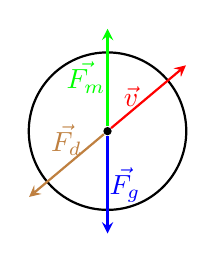
\begin{tikzpicture}
	%giganteska bola de fuego
	\node[fill=black,circle,inner sep=0pt, minimum size=3pt](center) at (0,0)
	{};
 \draw[thick] (center) circle (1);


	%speed
	\draw[thick, red, -stealth] (center) -- node[midway, left] {$\vec{v}$} (40:1.3);

	%gravitace
	\draw[thick, blue, -stealth] (center) --node[midway,right=-3pt] {$\vec{F_g}$} (-90:1.3);

	%drag
	\draw[thick,brown, -stealth] (center) --node[midway,left,above] {$\vec{F_d}$}
	 (220:1.3);

	%magnus force
	\draw[thick,green,-stealth] (center) --node[left=-3pt,midway] {$\vec{F_m}$} (90:1.3);


\end{tikzpicture}


 \caption{Síly působící na míček v letu}
 \label{fig:let-micku}
\end{figure}


\subsection{Rychlost}
\label{ssec:rychlost}
Rychlost, nebo lépe momentum, je síla zodpovědná za celý let. 


\subsection{Gravitační síla}
\label{ssec:gravitacni-sila}

Gravitační nebo také tíhová síla ($F_g$) je hned po rychlosti nejdůležitější sílou v
průběhu pohybu míčku. A spolu s rychlostí nejviditelněji tvoří rajektorii míčku.

Gravitace je také nejjednoduší na modelování. Dokud můžeme pro celou trajektorii
považovat Zemi za lokálně plochou, gravitační síla míří vždy směrem kolmů dolů.
Také její amplituda bývá většinou konstantní, protože není časté, že by míček
během letu měnil svojí váhu a změna v nadmořské výšce je zpravidla zanedbatelná.

Matematicky můžeme gravitaci vyjádřit jako:
\[
 F_g = G\frac{m}{h}
\]
Kde $G$ je gravitační konstanta, $m$ je váha míčku a $h$ je nadmořská výška.

Z této rovnice je ještě jednodušší nahlédnout na fakt, že gravitační síla je pro
náš případ konstantní. 


\subsection{Odpor vzduchu}
\label{ssec:odpor-vzduchu}

Odpor vzduchu ($F_d$) je často zanedbáván a to kvůli své relativní složitosti
oproti již zmíněné gravitační síle. Odpor vzduchu je totiž obecně závyslí na
rychlosti a ploše, která aktivně do vzduchu naráží. V případě míčku se mění jen
rychlost stále se ovšem jedná o složitou sílu na implementaci.

Směr odporu vzduchu je vždy opačný ke směru pohybu jak můžeme vidět na
\myref{obrázku}{fig:let-micku}. Velikost odporu závysí
kromě dalších koeficientů hlavně na kvadrátu rychlosti. 


\subsection{Magnusova síla}
\label{ssec:magnusova-sila}

Magnusova síla vzniká díky rotaci a vzájemnému třetí mezi míčkem a vzduchem.

